% NLP 2026 Project 1 extended abstract (CCN template from Moodle).
% Every number comes from the result files in results/ (see README.txt, section 7).
\documentclass[10pt,letterpaper]{article}

\usepackage{ccn}
\usepackage{pslatex}
\usepackage{apacite}
\usepackage{graphicx}
\usepackage{caption}
\usepackage{natbib}
\usepackage{float}

\usepackage[hidelinks]{hyperref}       % hyperlinks
\usepackage{url}            % simple URL typesetting
\usepackage{booktabs}       % professional-quality tables
\usepackage{amsfonts}       % blackboard math symbols
\usepackage{nicefrac}       % compact symbols for 1/2, etc.
\usepackage{microtype}      % microtypography
\usepackage{xcolor}         % colors
\usepackage{amsmath}
\usepackage{amssymb}
\usepackage{mathtools}
\usepackage{amsthm}
\usepackage[labelfont=bf, margin=0.8cm, font=sf]{caption}

% NeurIPS checklist answer macros (from neurips_2024.sty)
\newcommand{\answerYes}[1][]{\textcolor{blue}{[Yes] #1}}
\newcommand{\answerNo}[1][]{\textcolor{orange}{[No] #1}}
\newcommand{\answerNA}[1][]{\textcolor{gray}{[NA] #1}}

% Test-split numbers (from results/test_metrics.csv, evaluator fsl_test_class)
\newcommand{\TestGenZero}{0.958}
\newcommand{\TestTwoTen}{0.496}
\newcommand{\TestOneTen}{0.934}
\newcommand{\TestExtZero}{0.973}

\title{Does the Induction Circuit Warn of Model Collapse?}

\author{{\large \bf Jordan Tshibumbu (2453146)} \\ University of the Witwatersrand, 1 Jan Smuts Ave,\\ Braamfontein, Johannesburg, 2000, South Africa
  \AND {\large \bf Mivuyo Mpepo (2562730)} \\ University of the Witwatersrand, 1 Jan Smuts Ave,\\ Braamfontein, Johannesburg, 2000, South Africa
  \AND {\large \bf Okwukwechukwu Mbajiorgu (2430639)} \\ University of the Witwatersrand, 1 Jan Smuts Ave,\\ Braamfontein, Johannesburg, 2000, South Africa}

\begin{document}

\maketitle
\phantom{.}
\newpage
\phantom{.}
\newpage
\section{Abstract}
{
\bf
\looseness=-1
Model collapse is usually measured through outputs. We ask two questions: (Q1) when a transformer is trained recursively on its own outputs, does the induction circuit behind in-context learning degrade before behavior does and could it therefore act as an early warning of collapse? (Q2) can a collapsed model recover when trained on real data? Using the task and two-layer attention-only transformer from Singh et al. (2024), we relabel a fixed pool with each generation’s predictions, retrain for 10 generations, and track previous-token and induction heads at every checkpoint in both a base and an extended generative version. The circuit is not an early warning: loss and the probability assigned to in-context labels shift first, and the circuit fails together with accuracy, across two learning rates and three test thresholds. In the extended version, collapse appears in the next-symbol distribution while the circuit remains intact. Collapse is reversible and the circuit re-forms but recovery starts more slowly than training from scratch.
}
\begin{quote}
\small
\textbf{Keywords:}
model collapse; induction heads; mechanistic interpretability
\end{quote}

\section{Introduction} \label{Intro}
\looseness=-1
Models trained on data generated by earlier models lose the tails of the data distribution and eventually collapse \citep{shumailov2023curse,shumailov2024nature} but collapse is usually described in terms of outputs. Mechanistic interpretability identifies the circuits behind a behaviour \citep{conmy2023acdc}; the best-understood example is the induction circuit of in-context learning \citep{olsson2022induction,singh2024needs}. A layer-0 previous-token head copies each exemplar's identity onto the label token that follows it and a layer-1 induction head attends from the query to the label whose exemplar matches the query and copies it. If this circuit weakens before outputs degrade, it could flag collapse early. \textbf{Q1:} Does the circuit change before behaviour across generations? \textbf{Q2:} Does a collapsed model recover on real data, and does its circuit re-form?

\begin{figure*}[t]
  \centering
  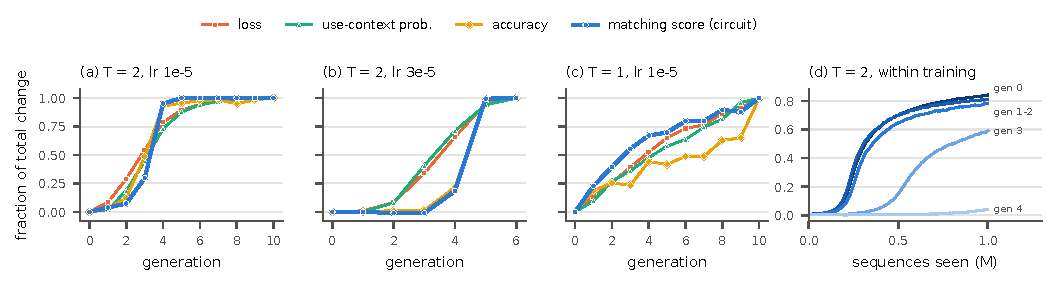
\includegraphics[width=\linewidth]{fig_main.pdf}
  \caption{\looseness=-1 \textbf{Behaviour changes before the circuit.} (a--c) For each measure, we plot its change from generation 0 as a fraction of its total change by the final generation; a curve that rises earlier changed earlier. Blue shows the matching score of the strongest induction head; orange, green, and yellow show behavioural measures. At $T{=}2$ (a; b at a better-converged learning rate), loss and use-context probability move first, while the circuit declines only alongside accuracy. At $T{=}1$ (c), nothing collapses within 10 generations, and the circuit weakens together with loss. (d) Matching score during training for $T{=}2$, generations 0--4: the circuit forms later in each generation and does not form at all in generation 4.}
  \label{fig:main}
\end{figure*}

\section{Methods}
\looseness=-1
\textbf{Task and model.} Each sequence contains two exemplar--label pairs and a query
($x_0y_0x_1y_1x_q$). The exemplars are frozen ResNet-18 embeddings of Omniglot characters
\citep{lake2015omniglot}; the query matches one exemplar and the model must output that exemplar's label. Labels are redrawn for each sequence from 5 tokens, so only the context can solve the task. We use the 2-layer, 8-head attention-only transformer and settings from \citet{singh2024needs} ($d{=}64$, rotary positions, batch 32, learning rate $10^{-5}$, seed 5). \textbf{Splits.} Training uses a fixed pool of $10^6$ sequences from the training characters. Validation (\texttt{fsl\_val\_rl}, unseen label assignments) is used for learning-rate selection and all analysis. Test (\texttt{fsl\_test\_class}, 100 unseen characters) is used only for final accuracy.
\textbf{Collapse.} Generation $n{-}1$ rewrites the query label of every pool row (argmax, or sampling from $\mathrm{softmax}(z/T)$, $T\in\{1,2\}$; in one $T{=}2$ setting, 10\% of rows stay real), and generation $n$ trains from scratch with the same initialisation; we run 10 generations. Argmax makes no errors and serves as the control; $T{=}2$ deliberately flattens the labels. In the extended version, the model also generates a next symbol (the query or the other exemplar, $p{=}0.5$) and its label and relabelling rewrites all three tokens. Its learning rate ($10^{-4}$) was chosen on validation loss from $\{1,3,10,30\}\times10^{-5}$.
\textbf{Circuit measures.} On 1,000 validation sequences, the matching score
$m_h=\frac{1}{B}\sum_b\big(A_h^{(b)}[q,\ell^{+}]-A_h^{(b)}[q,\ell^{-}]\big)$ of head $h$ is the query's attention to the correct label minus its attention to the other label. The previous-token score is a label's attention to its exemplar. We select the layer-1 head with the highest $m_h$ and the layer-0 heads scoring ${\geq}0.5$, confirm them by zero-ablation and track both the generation-0 head and each generation's strongest head ($m_{\max}$) since retraining can move the circuit.
\textbf{Early-warning test.} For each measure, we find the first generation that is worse than generation 0 by more than $z$ paired standard errors over the same sequences ($z{=}2,3,5$) and the first generation that changes by more than 10\%. The circuit gives an early warning only if it moves before accuracy, loss, and the probability on the in-context labels (use-context probability). Within training, we score every checkpoint ($10^4$ sequences apart).
\textbf{Q2.} Generation 10 of $T{=}2$ and $T{=}1$ then trains on $10^6$ more real sequences (with a fresh optimiser). Controls are: generation 0 trained longer (A), and $T{=}2$ generation 10 trained on its own pool (B).

\section{Results}
\looseness=-1
\textbf{Generation 0} reaches 0.997 validation and \TestGenZero{} test accuracy (all splits in Supplementary~E). Head 1:3 (layer 1, head 3) places 0.91 of the query's attention on the correct label (chance 0.2; $m{=}0.84$), supported by previous-token heads 0:1, 0:2, and 0:5 (0.85--0.90). Ablation shows the circuit is causal but redundant (Table~\ref{tab:ablation}): three other layer-1 heads also match ($m{=}0.56$--$0.70$). The extended model (\TestExtZero{} test accuracy) uses induction head 1:2 ($m{=}0.81$), and the same heads match the next symbol to its label ($m{=}0.80$).

\setlength{\belowcaptionskip}{-7pt}
\begin{table}[t]
\centering
\captionsetup{font=sf, width=0.95\linewidth, skip=5pt}
\caption{\looseness=-1 Generation-0 validation accuracy after zero-ablating heads.}
\small
\begin{tabular}{lcc}
\toprule
Heads ablated & Base & Extended\\
\midrule
none & 0.997 & 0.991\\
induction head & 0.974 & 0.898\\
all previous-token heads & 0.620 & 0.634\\
layer 1 except induction head & 0.955 & 0.891\\
all of layer 1 & 0.488 & 0.476\\
\bottomrule
\end{tabular}
\label{tab:ablation}
\end{table}
\setlength{\belowcaptionskip}{0pt}

\textbf{Q1: the circuit is not an early warning.} Under $T{=}2$, loss rises six-fold after one generation (0.025 to 0.159) while accuracy is still 0.980. By the 10\% criterion, loss moves at generation 1, use-context probability at 2, and $m_{\max}$ and accuracy together at 3 (Fig.~\ref{fig:main}a; with 10\% real data, loss at 1 and the rest at 3). The $z$-test flags the circuit and loss in the same generation for $z{=}2,3,5$; the circuit leads only accuracy, at strict thresholds, because accuracy barely moves near ceiling (Supplementary~B). Argmax shows no change. Backup heads fail first (layer-1 heads with $m{>}0.5$: 4 to 1 by generation 2, while the main head is still 0.78), then the main head fails together with accuracy. $T{=}1$ does not collapse (accuracy 0.954, $m_{\max}$ 0.74 at generation 10). Test accuracy at generation 10 is \TestTwoTen{} ($T{=}2$) and \TestOneTen{} ($T{=}1$). Within training, the circuit forms later each generation but accuracy is delayed just as much (50\% points $2.8/3.0/5.8$ vs $2.5/3.8/6.1\times10^5$ sequences in generations 0/2/3; Fig.~\ref{fig:main}d).
\textbf{Learning rate.} $3\times10^{-5}$ reached a lower validation loss than the $10^{-5}$ used ($0.0016\pm0.0007$ vs $0.025\pm0.003$). Repeating $T{=}2$ at $3\times10^{-5}$ strengthens the result: $m_{\max}$ stays at 0.90--0.91 through generation 3 while loss rises from 0.002 to 0.52 and use-context probability falls to 0.77; the circuit fails only at generation 4, together with accuracy (Fig.~\ref{fig:main}b).

\textbf{Extended version.} In the argmax control, the circuit moves to head 1:4 without any collapse, so tracking the generation-0 head raises a false alarm; $m_{\max}$ does not. Under $T{=}1$, query accuracy stays at 0.99, but the next-symbol distribution drifts: the spread of the per-sequence repeat share grows from 0.022 to 0.109 (0.024 if the model generalised), as each model copies each sequence's own share (correlation 0.90; Supplementary~C), and the in-context symbol probability falls from 0.98 to 0.87. The circuit does not follow ($m_{\max}$ dips to 0.72 and returns to 0.82).

\textbf{Q2: recovery.} On real data, the collapsed $T{=}2$ model returns to 0.991 accuracy and re-forms the circuit in head 1:3 ($m{=}0.85$, vs 0.94 for control A); $T{=}1$ recovers to 0.999 ($m{=}0.92$). Control B stays at chance (loss $\ln 5$). Recovery starts later than training from scratch (10/50/90\% of the rise at $2.2/3.4/5.9$ vs $0.8/2.5/4.6\times10^5$ sequences) but then rises as fast (10--90\%: $3.6$ vs $3.8\times10^5$; Table~\ref{tab:q2}).

\setlength{\belowcaptionskip}{-7pt}
\begin{table}[h]
\centering
\captionsetup{font=sf, width=0.95\linewidth, skip=5pt}
\caption{\looseness=-1 Q2: validation accuracy, induction head and its matching score after $10^6$ more sequences.}
\small
\begin{tabular}{lccc}
\toprule
Run & Acc. & Head & $m$\\
\midrule
A: generation 0, real data & 1.000 & 1:3 & 0.94\\
$T{=}1$ generation 10, real data & 0.999 & 1:3 & 0.92\\
$T{=}2$ generation 10, real data & 0.991 & 1:3 & 0.85\\
B: $T{=}2$ generation 10, own pool & 0.500 & -- & 0.00\\
\bottomrule
\end{tabular}
\label{tab:q2}
\end{table}
\setlength{\belowcaptionskip}{0pt}

\section{Discussion}
\looseness=-1
\textbf{Q1: no.} Under $T{=}2$, collapse begins with a loss of \emph{confidence}: trained on flattened labels, the model still attends to and predicts the correct label but it spreads probability across labels. Loss and use-context probability capture this; attention does not. The circuit fails only after most training labels are wrong (58\% in generation 4's pool at $3\times10^{-5}$). In the extended version, collapse occurs in a computation that the circuit does not cover so a circuit monitor must target the mechanism that actually degrades. \textbf{Q2: yes} but the collapsed model is a worse starting point than random weights, plausibly because it must first leave the uniform-prediction plateau (initial loss 1.59 ${\approx}\ln 5$; untested).

\textbf{Limitations.} We use one seed and a small synthetic task; the shared initialisation may explain re-formation in head 1:3; ablation is performed only at final checkpoints; the base learning rate was under-converged (the second rate was checked only for $T{=}2$); the test detects only decreases; and $T{=}1$ may collapse after 10 generations.

\section{Contribution Statements}
\looseness=-1
Jordan Tshibumbu reproduced the baseline of \citet{singh2024needs}, implemented the model-collapse pipeline for the base version, ran the base-version collapse experiments, and designed and implemented the extended version and its analysis scripts. Mivuyo Mpepo led Q1: she wrote the circuit-analysis code (identifying the previous-token and induction heads, tracking them across generations and within training, and implementing the early-warning test) and applied it to both versions. She also ran the extended-version experiments and wrote the report, \texttt{README.txt}, and \texttt{requirements.txt}. Okwukwechukwu Mbajiorgu led Q2 and the hyperparameter work, including the extended-version learning-rate selection, the base learning-rate check, and the robustness run at a second learning rate. He ran the Q2 recovery experiments and used the circuit measures to analyze circuit re-formation during recovery. All authors agree with this statement.
\bibliographystyle{apacite}

\setlength{\bibleftmargin}{.125in}
\setlength{\bibindent}{-\bibleftmargin}

\bibliography{references}

\onecolumn
\appendix
\section*{NeurIPS Paper Checklist}

\begin{enumerate}

\item {\bf Claims}
    \item[] Question: Do the main claims made in the abstract and introduction accurately reflect the paper's contributions and scope?
    \item[] Answer: \answerYes{} % Replace by \answerYes{}, \answerNo{}, or \answerNA{}.
    \item[] Justification: The abstract and introduction state the two questions, the setting (one synthetic in-context learning task, a two-layer attention-only transformer, one seed) and the main findings, which are reported in the Results with the numbers they rest on.
    \item[] Guidelines:
    \begin{itemize}
        \item The answer NA means that the abstract and introduction do not include the claims made in the paper.
        \item The abstract and/or introduction should clearly state the claims made, including the contributions made in the paper and important assumptions and limitations. A No or NA answer to this question will not be perceived well by the reviewers. 
        \item The claims made should match theoretical and experimental results, and reflect how much the results can be expected to generalize to other settings. 
        \item It is fine to include aspirational goals as motivation as long as it is clear that these goals are not attained by the paper. 
    \end{itemize}

\item {\bf Limitations}
    \item[] Question: Does the paper discuss the limitations of the work performed by the authors?
    \item[] Answer: \answerYes{} % Replace by \answerYes{}, \answerNo{}, or \answerNA{}.
    \item[] Justification: The Discussion has a Limitations paragraph: one seed, a small synthetic task, shared initialisation across generations, ablation only at final checkpoints, an under-converged base learning rate (checked at a second rate for $T{=}2$), a test that detects only decreases, and only 10 generations.
    \item[] Guidelines:
    \begin{itemize}
        \item The answer NA means that the paper has no limitation while the answer No means that the paper has limitations, but those are not discussed in the paper. 
        \item The authors are encouraged to create a separate "Limitations" section in their paper.
        \item The paper should point out any strong assumptions and how robust the results are to violations of these assumptions (e.g., independence assumptions, noiseless settings, model well-specification, asymptotic approximations only holding locally). The authors should reflect on how these assumptions might be violated in practice and what the implications would be.
        \item The authors should reflect on the scope of the claims made, e.g., if the approach was only tested on a few datasets or with a few runs. In general, empirical results often depend on implicit assumptions, which should be articulated.
        \item The authors should reflect on the factors that influence the performance of the approach. For example, a facial recognition algorithm may perform poorly when image resolution is low or images are taken in low lighting. Or a speech-to-text system might not be used reliably to provide closed captions for online lectures because it fails to handle technical jargon.
        \item The authors should discuss the computational efficiency of the proposed algorithms and how they scale with dataset size.
        \item If applicable, the authors should discuss possible limitations of their approach to address problems of privacy and fairness.
        \item While the authors might fear that complete honesty about limitations might be used by reviewers as grounds for rejection, a worse outcome might be that reviewers discover limitations that aren't acknowledged in the paper. The authors should use their best judgment and recognize that individual actions in favor of transparency play an important role in developing norms that preserve the integrity of the community. Reviewers will be specifically instructed to not penalize honesty concerning limitations.
    \end{itemize}

\item {\bf Theory Assumptions and Proofs}
    \item[] Question: For each theoretical result, does the paper provide the full set of assumptions and a complete (and correct) proof?
    \item[] Answer: \answerNA{} % Replace by \answerYes{}, \answerNo{}, or \answerNA{}.
    \item[] Justification: The paper makes no theoretical claims; the drift predictions in Supplementary C are standard binomial and Wright--Fisher variances used only as reference curves.
    \item[] Guidelines:
    \begin{itemize}
        \item The answer NA means that the paper does not include theoretical results. 
        \item All the theorems, formulas, and proofs in the paper should be numbered and cross-referenced.
        \item All assumptions should be clearly stated or referenced in the statement of any theorems.
        \item The proofs can either appear in the main paper or the supplemental material, but if they appear in the supplemental material, the authors are encouraged to provide a short proof sketch to provide intuition. 
        \item Inversely, any informal proof provided in the core of the paper should be complemented by formal proofs provided in appendix or supplemental material.
        \item Theorems and Lemmas that the proof relies upon should be properly referenced. 
    \end{itemize}

    \item {\bf Experimental Result Reproducibility}
    \item[] Question: Does the paper fully disclose all the information needed to reproduce the main experimental results of the paper to the extent that it affects the main claims and/or conclusions of the paper (regardless of whether the code and data are provided or not)?
    \item[] Answer: \answerYes{} % Replace by \answerYes{}, \answerNo{}, or \answerNA{}.
    \item[] Justification: Methods give the task, model, training settings, seeds (initialisation 5, pool 10, relabelling seed $n$ for generation $n$), relabelling rules, probe set, measures and test; README.txt lists the exact commands and Colab notebooks that produced every result.
    \item[] Guidelines:
    \begin{itemize}
        \item The answer NA means that the paper does not include experiments.
        \item If the paper includes experiments, a No answer to this question will not be perceived well by the reviewers: Making the paper reproducible is important, regardless of whether the code and data are provided or not.
        \item If the contribution is a dataset and/or model, the authors should describe the steps taken to make their results reproducible or verifiable. 
        \item Depending on the contribution, reproducibility can be accomplished in various ways. For example, if the contribution is a novel architecture, describing the architecture fully might suffice, or if the contribution is a specific model and empirical evaluation, it may be necessary to either make it possible for others to replicate the model with the same dataset, or provide access to the model. In general. releasing code and data is often one good way to accomplish this, but reproducibility can also be provided via detailed instructions for how to replicate the results, access to a hosted model (e.g., in the case of a large language model), releasing of a model checkpoint, or other means that are appropriate to the research performed.
        \item While NeurIPS does not require releasing code, the conference does require all submissions to provide some reasonable avenue for reproducibility, which may depend on the nature of the contribution. For example
        \begin{enumerate}
            \item If the contribution is primarily a new algorithm, the paper should make it clear how to reproduce that algorithm.
            \item If the contribution is primarily a new model architecture, the paper should describe the architecture clearly and fully.
            \item If the contribution is a new model (e.g., a large language model), then there should either be a way to access this model for reproducing the results or a way to reproduce the model (e.g., with an open-source dataset or instructions for how to construct the dataset).
            \item We recognize that reproducibility may be tricky in some cases, in which case authors are welcome to describe the particular way they provide for reproducibility. In the case of closed-source models, it may be that access to the model is limited in some way (e.g., to registered users), but it should be possible for other researchers to have some path to reproducing or verifying the results.
        \end{enumerate}
    \end{itemize}


\item {\bf Open access to data and code}
    \item[] Question: Does the paper provide open access to the data and code, with sufficient instructions to faithfully reproduce the main experimental results, as described in supplemental material?
    \item[] Answer: \answerYes{} % Replace by \answerYes{}, \answerNo{}, or \answerNA{}.
    \item[] Justification: All code (training, collapse pipeline, analysis, notebooks, figure script) and the result tables are submitted with the paper; the Omniglot embedding file used for training is included in the submitted repository, and README.txt explains how to run everything.
    \item[] Guidelines:
    \begin{itemize}
        \item The answer NA means that paper does not include experiments requiring code.
        \item Please see the NeurIPS code and data submission guidelines (\url{https://nips.cc/public/guides/CodeSubmissionPolicy}) for more details.
        \item While we encourage the release of code and data, we understand that this might not be possible, so “No” is an acceptable answer. Papers cannot be rejected simply for not including code, unless this is central to the contribution (e.g., for a new open-source benchmark).
        \item The instructions should contain the exact command and environment needed to run to reproduce the results. See the NeurIPS code and data submission guidelines (\url{https://nips.cc/public/guides/CodeSubmissionPolicy}) for more details.
        \item The authors should provide instructions on data access and preparation, including how to access the raw data, preprocessed data, intermediate data, and generated data, etc.
        \item The authors should provide scripts to reproduce all experimental results for the new proposed method and baselines. If only a subset of experiments are reproducible, they should state which ones are omitted from the script and why.
        \item At submission time, to preserve anonymity, the authors should release anonymized versions (if applicable).
        \item Providing as much information as possible in supplemental material (appended to the paper) is recommended, but including URLs to data and code is permitted.
    \end{itemize}


\item {\bf Experimental Setting/Details}
    \item[] Question: Does the paper specify all the training and test details (e.g., data splits, hyperparameters, how they were chosen, type of optimizer, etc.) necessary to understand the results?
    \item[] Answer: \answerYes{} % Replace by \answerYes{}, \answerNo{}, or \answerNA{}.
    \item[] Justification: Methods state the splits (training pool; validation \texttt{fsl\_val\_rl} with held-out label assignments for learning-rate selection and analysis; test \texttt{fsl\_test\_class} with held-out Omniglot classes), optimiser settings, learning-rate selection and pool sizes; Supplementary A gives the learning-rate sweeps.
    \item[] Guidelines:
    \begin{itemize}
        \item The answer NA means that the paper does not include experiments.
        \item The experimental setting should be presented in the core of the paper to a level of detail that is necessary to appreciate the results and make sense of them.
        \item The full details can be provided either with the code, in appendix, or as supplemental material.
    \end{itemize}

\item {\bf Experiment Statistical Significance}
    \item[] Question: Does the paper report error bars suitably and correctly defined or other appropriate information about the statistical significance of the experiments?
    \item[] Answer: \answerYes{} % Replace by \answerYes{}, \answerNo{}, or \answerNA{}.
    \item[] Justification: The early-warning test uses paired standard errors over the same 1,000 validation sequences, with thresholds $z=2,3,5$ and a 10\% effect-size criterion (Supplementary B); the learning-rate sweep reports standard errors. All results are from one seed, which we state as a limitation.
    \item[] Guidelines:
    \begin{itemize}
        \item The answer NA means that the paper does not include experiments.
        \item The authors should answer "Yes" if the results are accompanied by error bars, confidence intervals, or statistical significance tests, at least for the experiments that support the main claims of the paper.
        \item The factors of variability that the error bars are capturing should be clearly stated (for example, train/test split, initialization, random drawing of some parameter, or overall run with given experimental conditions).
        \item The method for calculating the error bars should be explained (closed form formula, call to a library function, bootstrap, etc.)
        \item The assumptions made should be given (e.g., Normally distributed errors).
        \item It should be clear whether the error bar is the standard deviation or the standard error of the mean.
        \item It is OK to report 1-sigma error bars, but one should state it. The authors should preferably report a 2-sigma error bar than state that they have a 96\% CI, if the hypothesis of Normality of errors is not verified.
        \item For asymmetric distributions, the authors should be careful not to show in tables or figures symmetric error bars that would yield results that are out of range (e.g. negative error rates).
        \item If error bars are reported in tables or plots, The authors should explain in the text how they were calculated and reference the corresponding figures or tables in the text.
    \end{itemize}

\item {\bf Experiments Compute Resources}
    \item[] Question: For each experiment, does the paper provide sufficient information on the computer resources (type of compute workers, memory, time of execution) needed to reproduce the experiments?
    \item[] Answer: \answerYes{} % Replace by \answerYes{}, \answerNo{}, or \answerNA{}.
    \item[] Justification: Each $10^6$-sequence training run took about 4--5 minutes on one NVIDIA T4 GPU (Google Colab); the extended, learning-rate, recovery and robustness experiments were about 30 such runs, and the 34 base-version runs were trained on an NVIDIA RTX 4050 laptop GPU. The circuit analysis took about 1 GPU-hour.
    \item[] Guidelines:
    \begin{itemize}
        \item The answer NA means that the paper does not include experiments.
        \item The paper should indicate the type of compute workers CPU or GPU, internal cluster, or cloud provider, including relevant memory and storage.
        \item The paper should provide the amount of compute required for each of the individual experimental runs as well as estimate the total compute. 
        \item The paper should disclose whether the full research project required more compute than the experiments reported in the paper (e.g., preliminary or failed experiments that didn't make it into the paper). 
    \end{itemize}
    
\item {\bf Code Of Ethics}
    \item[] Question: Does the research conducted in the paper conform, in every respect, with the NeurIPS Code of Ethics \url{https://neurips.cc/public/EthicsGuidelines}?
    \item[] Answer: \answerYes{} % Replace by \answerYes{}, \answerNo{}, or \answerNA{}.
    \item[] Justification: The work uses a public dataset of handwritten characters and synthetic labels, involves no human subjects or personal data, and conforms with the NeurIPS Code of Ethics.
    \item[] Guidelines:
    \begin{itemize}
        \item The answer NA means that the authors have not reviewed the NeurIPS Code of Ethics.
        \item If the authors answer No, they should explain the special circumstances that require a deviation from the Code of Ethics.
        \item The authors should make sure to preserve anonymity (e.g., if there is a special consideration due to laws or regulations in their jurisdiction).
    \end{itemize}


\item {\bf Broader Impacts}
    \item[] Question: Does the paper discuss both potential positive societal impacts and negative societal impacts of the work performed?
    \item[] Answer: \answerYes{} % Replace by \answerYes{}, \answerNo{}, or \answerNA{}.
    \item[] Justification: Positive: interpretability-based monitoring could help detect degradation when models are trained on generated data. Negative: none specific to this small synthetic study; we note in the Discussion that a negative result for one circuit should not be taken as evidence that monitoring is unnecessary.
    \item[] Guidelines:
    \begin{itemize}
        \item The answer NA means that there is no societal impact of the work performed.
        \item If the authors answer NA or No, they should explain why their work has no societal impact or why the paper does not address societal impact.
        \item Examples of negative societal impacts include potential malicious or unintended uses (e.g., disinformation, generating fake profiles, surveillance), fairness considerations (e.g., deployment of technologies that could make decisions that unfairly impact specific groups), privacy considerations, and security considerations.
        \item The conference expects that many papers will be foundational research and not tied to particular applications, let alone deployments. However, if there is a direct path to any negative applications, the authors should point it out. For example, it is legitimate to point out that an improvement in the quality of generative models could be used to generate deepfakes for disinformation. On the other hand, it is not needed to point out that a generic algorithm for optimizing neural networks could enable people to train models that generate Deepfakes faster.
        \item The authors should consider possible harms that could arise when the technology is being used as intended and functioning correctly, harms that could arise when the technology is being used as intended but gives incorrect results, and harms following from (intentional or unintentional) misuse of the technology.
        \item If there are negative societal impacts, the authors could also discuss possible mitigation strategies (e.g., gated release of models, providing defenses in addition to attacks, mechanisms for monitoring misuse, mechanisms to monitor how a system learns from feedback over time, improving the efficiency and accessibility of ML).
    \end{itemize}
    
\item {\bf Safeguards}
    \item[] Question: Does the paper describe safeguards that have been put in place for responsible release of data or models that have a high risk for misuse (e.g., pretrained language models, image generators, or scraped datasets)?
    \item[] Answer: \answerNA{} % Replace by \answerYes{}, \answerNo{}, or \answerNA{}.
    \item[] Justification: We release no data or models with a high risk of misuse.
    \item[] Guidelines:
    \begin{itemize}
        \item The answer NA means that the paper poses no such risks.
        \item Released models that have a high risk for misuse or dual-use should be released with necessary safeguards to allow for controlled use of the model, for example by requiring that users adhere to usage guidelines or restrictions to access the model or implementing safety filters. 
        \item Datasets that have been scraped from the Internet could pose safety risks. The authors should describe how they avoided releasing unsafe images.
        \item We recognize that providing effective safeguards is challenging, and many papers do not require this, but we encourage authors to take this into account and make a best faith effort.
    \end{itemize}

\item {\bf Licenses for existing assets}
    \item[] Question: Are the creators or original owners of assets (e.g., code, data, models), used in the paper, properly credited and are the license and terms of use explicitly mentioned and properly respected?
    \item[] Answer: \answerYes{} % Replace by \answerYes{}, \answerNo{}, or \answerNA{}.
    \item[] Justification: We use and cite the code and Omniglot embeddings of \citet{singh2024needs} and the Omniglot dataset \citep{lake2015omniglot}; their licence terms are those stated in the original repositories.
    \item[] Guidelines:
    \begin{itemize}
        \item The answer NA means that the paper does not use existing assets.
        \item The authors should cite the original paper that produced the code package or dataset.
        \item The authors should state which version of the asset is used and, if possible, include a URL.
        \item The name of the license (e.g., CC-BY 4.0) should be included for each asset.
        \item For scraped data from a particular source (e.g., website), the copyright and terms of service of that source should be provided.
        \item If assets are released, the license, copyright information, and terms of use in the package should be provided. For popular datasets, \url{paperswithcode.com/datasets} has curated licenses for some datasets. Their licensing guide can help determine the license of a dataset.
        \item For existing datasets that are re-packaged, both the original license and the license of the derived asset (if it has changed) should be provided.
        \item If this information is not available online, the authors are encouraged to reach out to the asset's creators.
    \end{itemize}

\item {\bf New Assets}
    \item[] Question: Are new assets introduced in the paper well documented and is the documentation provided alongside the assets?
    \item[] Answer: \answerYes{} % Replace by \answerYes{}, \answerNo{}, or \answerNA{}.
    \item[] Justification: The new code (collapse pipeline, extended version, analysis package \texttt{interp/}, notebooks) is documented in README.txt and in docstrings, and is submitted with the paper.
    \item[] Guidelines:
    \begin{itemize}
        \item The answer NA means that the paper does not release new assets.
        \item Researchers should communicate the details of the dataset/code/model as part of their submissions via structured templates. This includes details about training, license, limitations, etc. 
        \item The paper should discuss whether and how consent was obtained from people whose asset is used.
        \item At submission time, remember to anonymize your assets (if applicable). You can either create an anonymized URL or include an anonymized zip file.
    \end{itemize}

\item {\bf Crowdsourcing and Research with Human Subjects}
    \item[] Question: For crowdsourcing experiments and research with human subjects, does the paper include the full text of instructions given to participants and screenshots, if applicable, as well as details about compensation (if any)? 
    \item[] Answer: \answerNA{} % Replace by \answerYes{}, \answerNo{}, or \answerNA{}.
    \item[] Justification: No crowdsourcing or human subjects were involved.
    \item[] Guidelines:
    \begin{itemize}
        \item The answer NA means that the paper does not involve crowdsourcing nor research with human subjects.
        \item Including this information in the supplemental material is fine, but if the main contribution of the paper involves human subjects, then as much detail as possible should be included in the main paper. 
        \item According to the NeurIPS Code of Ethics, workers involved in data collection, curation, or other labor should be paid at least the minimum wage in the country of the data collector. 
    \end{itemize}

\item {\bf Institutional Review Board (IRB) Approvals or Equivalent for Research with Human Subjects}
    \item[] Question: Does the paper describe potential risks incurred by study participants, whether such risks were disclosed to the subjects, and whether Institutional Review Board (IRB) approvals (or an equivalent approval/review based on the requirements of your country or institution) were obtained?
    \item[] Answer: \answerNA{} % Replace by \answerYes{}, \answerNo{}, or \answerNA{}.
    \item[] Justification: No human subjects were involved, so no IRB approval was required.
    \item[] Guidelines:
    \begin{itemize}
        \item The answer NA means that the paper does not involve crowdsourcing nor research with human subjects.
        \item Depending on the country in which research is conducted, IRB approval (or equivalent) may be required for any human subjects research. If you obtained IRB approval, you should clearly state this in the paper. 
        \item We recognize that the procedures for this may vary significantly between institutions and locations, and we expect authors to adhere to the NeurIPS Code of Ethics and the guidelines for their institution. 
        \item For initial submissions, do not include any information that would break anonymity (if applicable), such as the institution conducting the review.
    \end{itemize}

\end{enumerate}


\clearpage
\section*{AI Ethics Statement (Faculty of Science)}
Generative AI was used in this project. Claude (Anthropic), accessed through the Claude application, helped write and test the analysis code (\texttt{interp/}), the Google Colab notebooks, and the figure script; interpret the experimental results and draft and edit this report, \texttt{README.txt} and the checklist answers.

We checked the AI-assisted output in several ways. The analysis code has unit tests (\texttt{test\_interp\_heads.py}), including one that reproduces the validation accuracy logged by the training code for generation 0 (0.997) from our own forward pass. The argmax control confirmed that the analysis reports no change when nothing changes. We traced every number in the report to a result file listed in \texttt{README.txt} and checked every reference against the publisher's page. We discarded AI suggestions that did not pass these checks. For example, following the generation-0 head in the extended version produced false alarms, which the argmax control exposed; we therefore changed the analysis to track the strongest head.

We take full responsibility for all code and writing submitted, including any errors.

\clearpage
\section*{Supplementary material}
% =====================================================================
% OPTIONAL SUPPLEMENTARY MATERIAL (goes after the AI Ethics Statement, per the brief)
% Generated from results/ by a script (numbers copied, not retyped). Needs \usepackage{float} for [H].
% =====================================================================
\subsection*{A. Learning-rate selection (validation set \texttt{fsl\_val\_rl})}
\begin{table}[H]\centering\small
\begin{tabular}{lccc}\toprule
Base, gen 0 & val.\ loss & SE & in-context acc.\\\midrule
$10^{-5}$ (used) & 0.0248 & 0.0025 & 0.997\\
$3{\times}10^{-6}$ & 0.3765 & 0.0119 & 0.841\\
$3{\times}10^{-5}$ & 0.0016 & 0.0007 & 1.000\\
\bottomrule\end{tabular}\\[6pt]
\begin{tabular}{lcccc}\toprule
Extended, gen 0 & total loss & symbol loss & query acc. & next-label acc.\\\midrule
$10^{-5}$ & 1.374 & 1.083 & 0.956 & 0.953\\
$3{\times}10^{-5}$ & 0.876 & 0.787 & 0.985 & 0.991\\
$10^{-4}$ (used) & 0.796 & 0.757 & 0.991 & 0.996\\
$3{\times}10^{-4}$ & 12.013 & 0.758 & 0.694 & 0.652\\
\bottomrule\end{tabular}
\caption{Validation results after $10^6$ sequences. The symbol-loss floor for $p{=}0.5$ is $\ln 2\approx0.693$.}
\end{table}

\subsection*{B. Early-warning test for the strongest induction head ($m_{\max}$)}
First generation at which each measure is worse than generation 0 by more than $z$ paired standard
errors, and the first at which it changes by more than 10\%; ``--'' means never within the run.
\begin{table}[H]\centering\small
\begin{tabular}{llccccc}\toprule
Condition & Behaviour & $z{=}2$ & $z{=}3$ & $z{=}5$ & $>10\%$ & $m_{\max}$ at $>10\%$\\
 & & circ./beh. & circ./beh. & circ./beh. & beh. & \\\midrule
$T{=}2$ & accuracy & 1/1 & 1/1 & 1/2 & 3 & 3\\
 & loss & 1/1 & 1/1 & 1/1 & 1 & 3\\
 & use-context & 1/1 & 1/1 & 1/1 & 2 & 3\\
\midrule
$T{=}2$, 10\% real & accuracy & 1/1 & 1/1 & 1/2 & 3 & 3\\
 & loss & 1/1 & 1/1 & 1/1 & 1 & 3\\
 & use-context & 1/1 & 1/1 & 1/1 & 3 & 3\\
\midrule
$T{=}1$ & accuracy & 1/1 & 1/2 & 1/8 & -- & 8\\
 & loss & 1/1 & 1/1 & 1/1 & 1 & 8\\
 & use-context & 1/1 & 1/1 & 1/1 & -- & 8\\
\midrule
argmax & accuracy & --/-- & --/-- & --/-- & -- & --\\
 & loss & --/-- & --/-- & --/-- & -- & --\\
 & use-context & --/-- & --/-- & --/-- & -- & --\\
\midrule
$T{=}2$, lr $3{\times}10^{-5}$ & accuracy & & 4/4 & & 4 & 4\\
 & loss & & 4/1 & & 1 & 4\\
 & use-context & & 4/1 & & 3 & 4\\
\midrule
ext.\ $T{=}1$ & accuracy & & 1/-- & & -- & 1\\
 & loss & & 1/-- & & 2 & 1\\
 & use-context & & 1/1 & & -- & 1\\
\midrule
ext.\ argmax & accuracy & & --/-- & & -- & --\\
 & loss & & --/-- & & 2 & --\\
 & use-context & & --/1 & & -- & --\\
\bottomrule\end{tabular}
\caption{Lower block: only $z{=}3$ was run. In the extended version a 10\% change in loss is a change of
about 0.002 (loss $\approx0.02$), so that column is not meaningful there.}
\end{table}

\subsection*{C. Extended version, $T{=}1$: next-symbol drift}
\begin{table}[H]\centering\small
\begin{tabular}{rcccccc}\toprule
Pool & out-of-context & repeat share & spread (obs.) & spread if & spread if & corr.\ with own\\
gen & symbols & (in context) & & generalising & memorising & training share\\\midrule
0 & 0.000 & 0.500 & 0.022 & 0.021 & 0.021 & --\\
1 & 0.020 & 0.515 & 0.041 & 0.022 & 0.041 & 0.03\\
2 & 0.034 & 0.522 & 0.058 & 0.022 & 0.058 & 0.57\\
4 & 0.058 & 0.543 & 0.081 & 0.023 & 0.089 & 0.82\\
6 & 0.078 & 0.558 & 0.092 & 0.023 & 0.114 & 0.86\\
8 & 0.097 & 0.568 & 0.102 & 0.024 & 0.135 & 0.88\\
10 & 0.114 & 0.572 & 0.109 & 0.024 & 0.152 & 0.90\\
\bottomrule\end{tabular}
\caption{Pool $g$ is written by model $g{-}1$. Spread: variance across sequences of the share of copies
whose next symbol repeats the query (about 12.8 copies per sequence).}
\end{table}

\subsection*{D. Generation-0 heads}
\begin{figure}[H]\centering
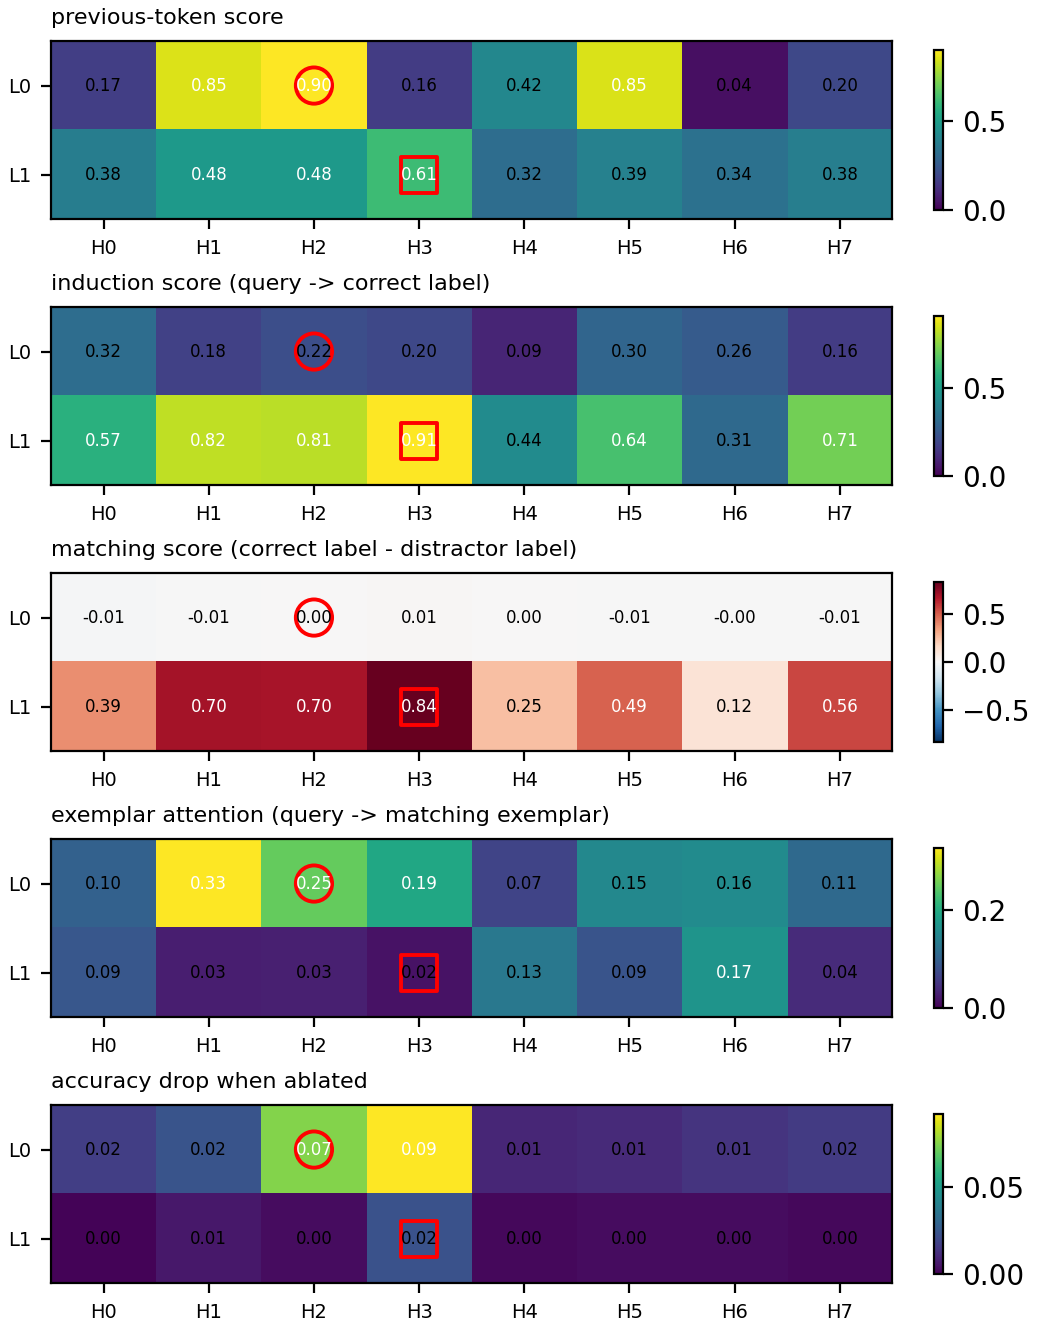
\includegraphics[width=0.48\linewidth]{gen0_head_heatmaps_base.png}\hfill
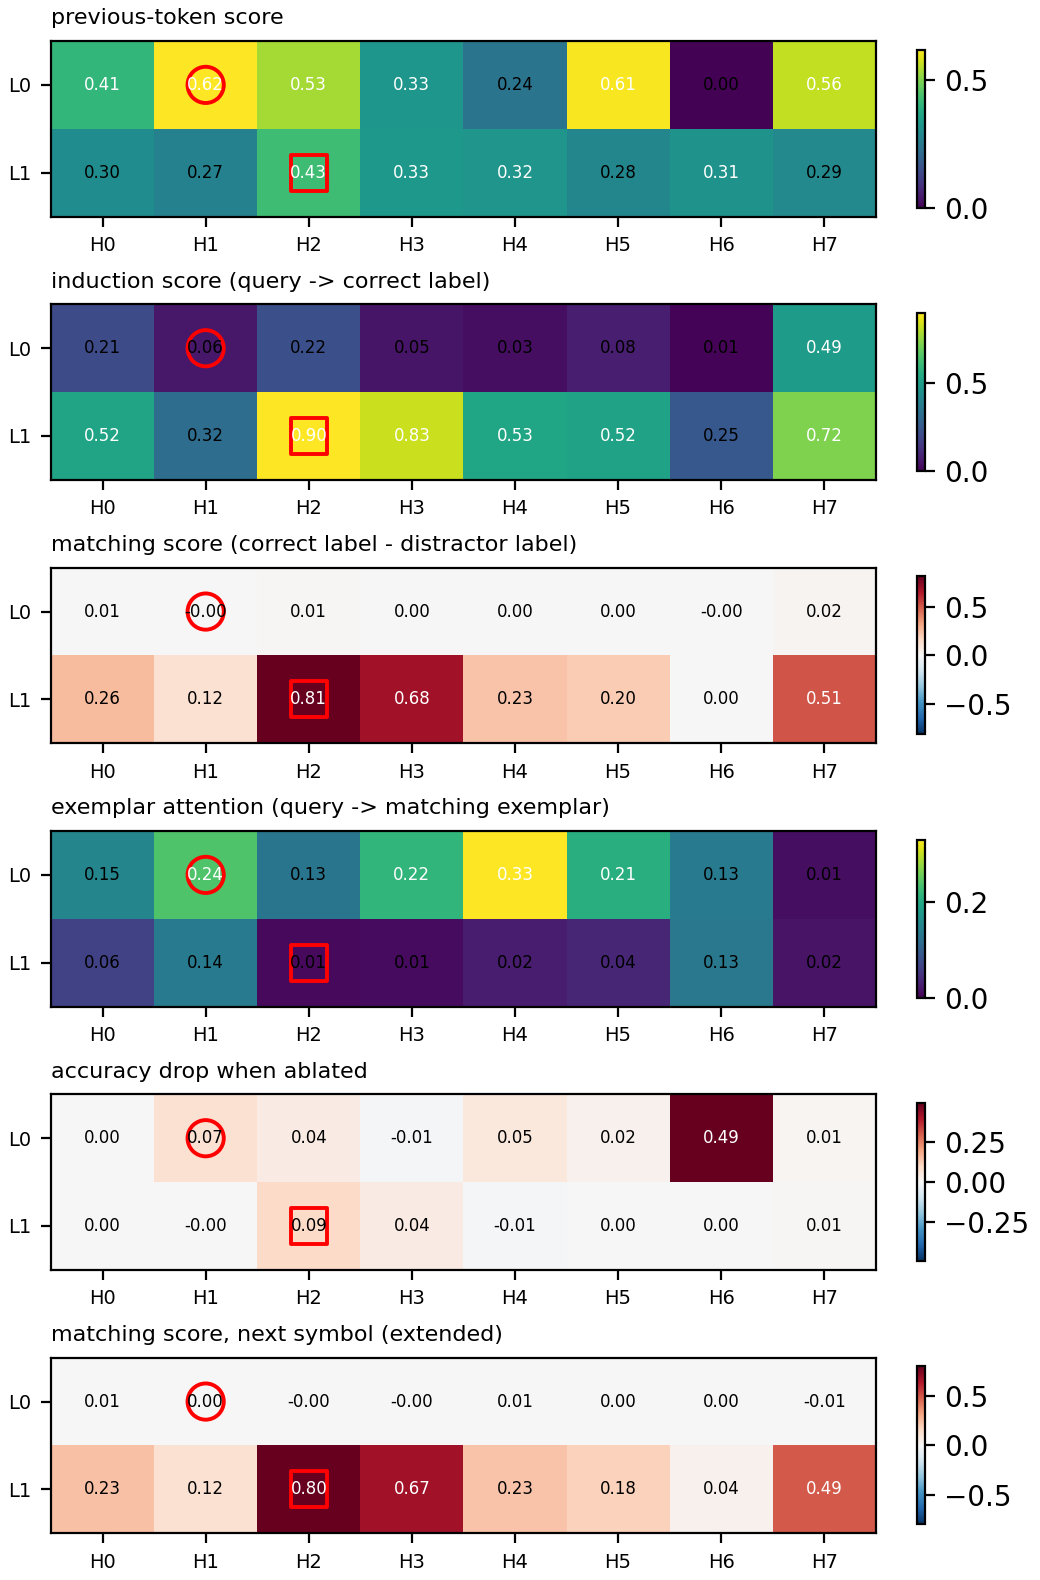
\includegraphics[width=0.48\linewidth]{gen0_head_heatmaps_ext.png}
\caption{Head scores and single-head ablation of the generation-0 model, base (left) and extended
(right). Circle: chosen previous-token head; square: chosen induction head.}
\end{figure}

\subsection*{E. Accuracy on the training, validation and test sets}
\begin{table}[H]\centering\small
\begin{tabular}{lcccc}\toprule
Run (final checkpoint) & train & validation & train chars., new exemplars & test (held-out chars.)\\\midrule
base generation 0 & 1.000 & 0.997 & 0.865 & 0.958\\
base $T{=}2$, generation 10 & 0.531 & 0.495 & 0.498 & 0.496\\
base $T{=}2$ (10\% real), generation 10 & 0.508 & 0.469 & 0.514 & 0.498\\
base $T{=}1$, generation 10 & 0.997 & 0.954 & 0.866 & 0.934\\
base argmax, generation 3 & 1.000 & 0.997 & 0.865 & 0.958\\
base generation 0, lr $3{\times}10^{-5}$ & 1.000 & 1.000 & 0.898 & 0.974\\
extended generation 0 & 1.000 & 0.991 & 0.863 & 0.973\\
extended $T{=}1$, generation 10 & 0.998 & 0.992 & 0.876 & 0.986\\
\bottomrule\end{tabular}
\caption{In-context accuracy from the training logs (\texttt{fsl\_train}, \texttt{fsl\_val\_rl},
\texttt{fsl\_train\_valex}, \texttt{fsl\_test\_class}); source \texttt{results/test\_metrics.csv}.
Chance is 0.5. The test set confirms the validation results: collapsed models are at chance on unseen
characters too.}
\end{table}


\end{document}
